% Load before IEEEtran to avoid XeTeX TU/Times font substitutions.
\RequirePackage[T1]{fontenc}
\documentclass[conference,a4paper]{IEEEtran}
\IEEEoverridecommandlockouts

% Packages retained from the manuscript; duplicate/conflicting imports removed.
\usepackage{cite}
\usepackage{float}
\usepackage{amsmath,amssymb,amsfonts}
\usepackage{mathtools}
\usepackage{algorithm}
\usepackage{algpseudocode}
\usepackage{graphicx}
\usepackage{textcomp}
\usepackage{xcolor}
\usepackage{booktabs}
\usepackage{tabularx}
\usepackage{array}
\usepackage{nicematrix}
\usepackage{balance}
\usepackage{enumitem}
\usepackage{tikz}
\usepackage{bm}
\usepackage{lipsum}
\usetikzlibrary{shapes.geometric}
\usepackage[hidelinks]{hyperref}

\algrenewcommand\algorithmicrequire{\textbf{Input:}}
\algrenewcommand\algorithmicensure{\textbf{Output:}}
\newtheorem{coro}{Corollary}
\newtheorem{theo}{Theorem}
\newtheorem{prop}{Proposition}
\newtheorem{remark}{Remark}
\newtheorem{example}{Example}
\newtheorem{lemma}{Lemma}
\newtheorem{defin}{Definition}
\hypersetup{breaklinks=true,citecolor=black,colorlinks=true,
            linkcolor=black,urlcolor=blue}
\setcounter{MaxMatrixCols}{30}

\title{Mobility-Aware UAV Positioning and Secret Key Rate Optimization for HAP--UAV CV-QKD}
\author{\IEEEauthorblockN{TBD\IEEEauthorrefmark{1},
TBD\IEEEauthorrefmark{2}}
\IEEEauthorblockA{\IEEEauthorrefmark{1}XXX}
\IEEEauthorblockA{\IEEEauthorrefmark{2}Computer Communications Laboratory,
The University of Aizu, Aizuwakamatsu 965-8580, Japan}}


\begin{document}
\maketitle
\begin{abstract}
This provisional internal-review study examines source selection and UAV positioning for a cloud-affected HAP--UAV discrete-modulated CV-QKD model. A finite catalog of 233 exact-source ensembles defines a common location-dependent numerical rate map. An offline stationary benchmark, a current-slot Greedy policy, and finite-horizon dynamic programming (DP) are compared under identical cloud realizations and speed constraints. Across 100 paired missions, expanding the candidate set from 10 to 100 raises the mean DP penalized objective by 11.41\%. At blockage probability 0.8, mean zero-rate unavailability is 24.60\%, 16.53\%, and 4.07\% for Stationary, Greedy, and DP, respectively. At the representative penalty, DP reduces travel by 88.37\% relative to zero penalty while reducing mean usable rate by 0.515\%. These are conditional manuscript-model outputs: the recorded two-dimensional mutual information and homodyne Holevo expression do not specify a consistent Bob measurement. The results characterize the saved numerical optimization and do not establish physical quantum security.
\end{abstract}
\begin{IEEEkeywords}
Continuous-variable quantum key distribution, UAV, high-altitude platform, cloud blockage, probabilistic shaping, dynamic programming.
\end{IEEEkeywords}
\noindent\textbf{Internal review only.} Security-model correction and author review remain pending. Status:\\
{\footnotesize\texttt{UNVALIDATED\_SECURITY\_MODEL};}\\
{\footnotesize\texttt{NOT\_READY\_FOR\_PUBLICATION\_SCALE\_RUNS}.}
\section{HAP--UAV CV-QKD System and Problem Formulation}
\label{sec:system}
\subsection{Mobility-Aware UAV Positioning and SKR Optimization}
We consider one UAV at a fixed altitude over a $1\,\mathrm{km}\times
1\,\mathrm{km}$ area, discretized into $J$ candidate positions
$\mathcal Q=\{\mathbf q_j\}_{j=1}^J$. The mission has $N_t$ slots of
duration $\Delta t$. Let $c_{j,n}\in\{0,1\}$ indicate cloud blockage
(one means blocked). The matrix $\mathbf C=[c_{j,n}]$ contains spatially
and temporally correlated Bernoulli states. P2 and P3 know the complete
matrix and are offline benchmarks; Greedy observes only the current slot.

For an unblocked link, the recorded manuscript-style raw rate is
\begin{equation}
 K_j(\nu,V_A)=\beta_{\rm rec}I_{AB,j}^{2D}(\nu,V_A)-\chi_{BE,j}(\nu,V_A).
 \label{eq:raw}
\end{equation}
Equation~\eqref{eq:raw} is retained as a conditional numerical metric,
subject to the measurement-consistency limitations below.

\section{Recorded Physical-Layer Model}
Alice sends the coherent-state ensemble $\{p_k,\alpha_k\}_{k=1}^{256}$.
With $[\hat x,\hat p]=2i$ and vacuum quadrature variance one, the
normalization is $V_A=2\sum_kp_k|\alpha_k|^2=2\bar n$.
The source moments $C_s,w_s$ are computed from this same ensemble;
the subscript distinguishes them from the cloud matrix.
For clear-sky power transmittance $\eta$, the saved evaluator uses
\begin{align*}
 \eta_f&=\langle\sqrt\eta\rangle^2,\\
 N=\eta_f\xi_f&=(\langle\eta\rangle-\eta_f)V_A
                  +\xi_{\rm ch}\langle\eta\rangle,\\
 V&=1+V_A,\qquad W=1+\eta_fV_A+N,\\
 Z&=2\sqrt{\eta_f}C_s-\sqrt{2Nw_s}.
\end{align*}
The convention is $\xi_n=\xi_{\rm ch}$. The additive $N$ is
output-referred excess noise; loss-induced vacuum is already included
in $W$'s unit baseline. The active detector is ideal (efficiency one,
electronic noise zero). No imperfect trusted-detector claim is made.
The clear-sky distribution retains a separate angle-of-arrival outage
atom at $\eta=0$ and its active density on $[0,1]$, without renormalizing.
Moment reduction at the covariance level has a precedent for Gaussian
modulation~\cite{usenko2012}; it is not an identity for the full
discrete-input fading likelihood.

\section{SKR Performance Analysis}
\subsection{Recorded Rate and Security Boundary}
\label{sec:security}
Specifically, the saved MI kernel uses the normalized likelihood
\[
 p_{\rm num}(\mathbf y|k)=\frac{
 \exp[-\|\mathbf y-2\sqrt{\eta_f}(\Re\alpha_k,\Im\alpha_k)\|^2/
                 (2(1+N))]}{2\pi(1+N)}
\]
and integrates both real components to obtain $I_{AB}^{2D}$.
The Holevo branch uses the standard-form covariance with entries
$V,W,Z$ and the \emph{homodyne} conditional eigenvalue
\[
 \nu_3^{\rm hom}=\sqrt{V(V-Z^2/W)}.
\]
These two branches do not specify one consistent single-mode Bob
measurement: a homodyne outcome has one quadrature, while joint
measurement of both quadratures adds measurement vacuum. The
measurement-dependent Holevo expressions are explicitly different
in~\cite{denys2021}. Consequently, all reported ``usable SKR'' values
are conditional outputs of the recorded manuscript model, not
established achievable secret-key rates.

Further, evaluating only $Z_-$ does not establish the worst-case
Holevo value over all admissible correlations; the general
interval-maximization caveat in~\cite[Sec.~4, footnotes 11--12]{denys2021}
also applies. A consistent measurement/noise specification, admissible
correlation treatment, parameter estimation, and fading/outage
conditioning protocol require author review. No correction is applied
to the historical numerical results in this manuscript revision.


\typeout{REVISION_LAYOUT textheight=\the\textheight;columnwidth=\the\columnwidth;textwidth=\the\textwidth;topmargin=\the\topmargin;headheight=\the\headheight;headsep=\the\headsep;voffset=\the\voffset}
\subsection{SKR Performance Optimization}
\label{sec:optimization}
\label{sec:method}
Although Maxwell--Boltzmann (MB) shaping improves numerical source
performance, cloud blockage also makes the usable rate depend on UAV
position. A fixed position can remain blocked, whereas movement exploits
spatial and temporal cloud variations at an additional travel cost.
We therefore consider source selection, stationary positioning, and
mobility-aware trajectory planning in sequence.

For position $j$, the MB parameter $\nu$ and modulation variance $V_A$
are selected from an exact-source catalog $\mathcal G$:
\begin{equation}
 \mathcal P_1:\quad K_j^\star=
 \left[\max_{(\nu,V_A)\in\mathcal G}K_j(\nu,V_A)\right]^+.
 \label{eq:p1}
\end{equation}
The catalog contains 197 MB and 36 uniform 256-QAM ensembles, each with
its own exact source moments. Raw rates are maximized before clipping;
optimality is restricted to this finite catalog. Under complete cloud
blockage, define $S_{j,n}=(1-c_{j,n})K_j^\star$. The optimal stationary
offline benchmark is
\begin{equation}
 \mathcal P_2:\quad j_{\rm fix}^\star=
 \arg\max_j\frac{1}{N_t}\sum_{n=1}^{N_t}S_{j,n}.
 \label{eq:p2}
\end{equation}
For $j_n\in\{1,\ldots,J\}$ and
$d_{i,j}=\|\mathbf q_i-\mathbf q_j\|_2$, the main mobility problem is
\begin{align}
 \mathcal P_3:\quad \max_{\{j_n\}}\quad&
 \frac{1}{N_t}\sum_{n=1}^{N_t}S_{j_n,n}
 -\frac{\lambda}{D_{\rm ref}}\sum_{n=2}^{N_t}d_{j_{n-1},j_n}
 \label{eq:p3}\\
 \mathrm{s.t.}\quad& d_{j_{n-1},j_n}\le v_{\max}\Delta t,
 \quad n=2,\ldots,N_t.\nonumber
\end{align}
The objective $U=\overline K-\lambda D/D_{\rm ref}$ balances mean usable
rate and total travel distance, where $\lambda\ge0$ has units of bit/use.
The constraint enforces the speed limit. Staying and free initial placement
are allowed, without deployment or return cost. Distance is a mobility-cost
surrogate rather than a calibrated propulsion-energy model.

Finite search solves P1; P2 compares the $J$ mission means. For P3, let
$\mathcal N(j)=\{i:d_{i,j}\le v_{\max}\Delta t\}$ include staying.
Dynamic programming (DP) retains the best accumulated score ending at $j$:
\begin{align}
 F_1(j)&=S_{j,1},\label{eq:dp_init}\\
 F_n(j)&=S_{j,n}+\max_{i\in\mathcal N(j)}
 \left[F_{n-1}(i)-\frac{N_t\lambda}{D_{\rm ref}}d_{i,j}\right].
 \label{eq:dp}
\end{align}
Algorithm~\ref{alg:dp} stores maximizing predecessors and backtracks from
the best terminal state, yielding $U^\star=\max_jF_{N_t}(j)/N_t$.
It finds the global optimum over the finite position grid for a known
cloud sequence, in $O(N_tJ^2)$ time with $O(N_tJ)$ backpointers.
As a current-slot baseline, Greedy starts at
$j_1^{\rm G}\in\arg\max_jS_{j,1}$ and selects
\begin{equation}
 j_n^{\rm G}\in\arg\max_{j\in\mathcal N(j_{n-1}^{\rm G})}
 \left[S_{j,n}-\frac{N_t\lambda}{D_{\rm ref}}d_{j_{n-1}^{\rm G},j}\right].
 \label{eq:greedy}
\end{equation}
It uses no future cloud states. P2 and DP are offline benchmarks.
On the same instance, DP attains an objective no smaller than P2 or Greedy,
but need not maximize availability or unpenalized rate. Its advantage also
reflects future information and initial-position selection.

\begin{algorithm}[t]
\caption{Dynamic Programming for Mobility-Aware UAV Positioning}
\label{alg:dp}
\begin{algorithmic}[1]
\Require Positions $\mathcal Q$, distances $d_{i,j}$, rates $S_{j,n}$;
\Statex \hspace{\algorithmicindent} $N_t$, $v_{\max}$, $\Delta t$, $\lambda$, $D_{\rm ref}$
\Ensure Trajectory $\{j_n^\star\}_{n=1}^{N_t}$ and objective $U^\star$
\State Set $F_1(j)\gets S_{j,1}$ for all $j$
\For{$n=2,\ldots,N_t$}
  \For{$j=1,\ldots,J$}
    \State Evaluate all $i\in\mathcal N(j)$ in~\eqref{eq:dp}
    \State Store a maximizer $b_n(j)$; update $F_n(j)$
  \EndFor
\EndFor
\State $j_{N_t}^\star\gets\arg\max_jF_{N_t}(j)$;
\Statex \hspace{\algorithmicindent} $U^\star\gets F_{N_t}(j_{N_t}^\star)/N_t$
\For{$n=N_t,\ldots,2$}
  \State $j_{n-1}^\star\gets b_n(j_n^\star)$
\EndFor
\State \Return $\{j_n^\star\}_{n=1}^{N_t}$, $U^\star$
\end{algorithmic}
\end{algorithm}

\section{Numerical Results \& Discussions}
\label{sec:numerical}
% The requested replacement figures retain numbers 2 and 3 in this revision.
% No earlier system illustration exists in the authenticated source snapshot.
\setcounter{figure}{1}
We evaluate the saved finite-catalog and positioning results under the
synthetic configuration in Table~\ref{tab:parameters}. Gaussian-copula
clouds have latent covariance $\exp(-d_{i,j}/\ell)$ and AR(1) coefficient
$\rho$. Methods share 100 paired missions; bands show saved pointwise
95\% whole-mission bootstrap intervals. Zero-rate unavailability counts
slots with $S=0$, without an engineering threshold. All rates retain the
measurement-consistency limitations of Section~\ref{sec:security}.

\begin{table}[t]
\caption{System Parameters of the Synthetic Mobility Experiment}
\label{tab:parameters}
\centering
\footnotesize
\begin{tabular}{@{}llll@{}}
\toprule
Parameter & Value & Parameter & Value\\
\midrule
HAP altitude & 20 km & UAV altitude & 1 km\\
Wavelength & 1550 nm & Full divergence & $233\,\mu$rad\\
Rx diameter & 0.08 m & $\beta_{\rm rec}$ & 0.95\\
$\xi_{\rm ch}$ & 0.0186 SNU & Detector & Ideal\\
Flight region & $1\times1$ km$^2$ & Positions $J$ & 100\\
Slots $N_t$ & 30 & Slot $\Delta t$ & 20 s\\
$v_{\max}$ & 15 m/s & $D_{\rm ref}$ & 1000 m\\
Cloud $p$ & 0.4 & Missions & 100\\
Spatial $\ell$ & 250 m & Latent $\rho$ & 0.9\\
\bottomrule
\end{tabular}
\end{table}

\begin{figure}[t]
\centering
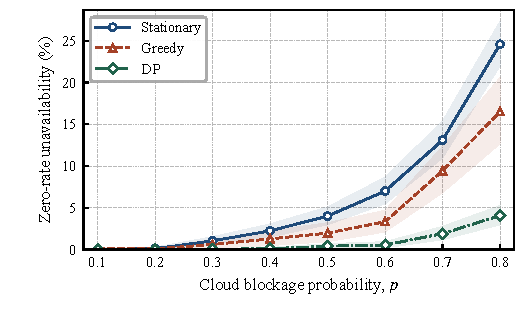
\includegraphics[width=\columnwidth]{figures/fig2_cloud_unavailability.pdf}
\caption{Cloud blockage probability versus zero-rate unavailability
at $\lambda_{\rm ref}$ for Stationary, Greedy, and DP.}
\label{fig:cloud}
\end{figure}

Fig.~\ref{fig:cloud} illustrates increasing unavailability with cloud
blockage. At $p=0.8$, Stationary, Greedy, and DP attain 24.60\%,
16.53\%, and 4.07\%, respectively. DP uses future cloud information
to route toward clear locations, reducing observed unavailability;
this is an offline planning benefit, not an implemented prediction system.
The optimized objective does not directly count available slots.

\begin{figure*}[t]
\centering
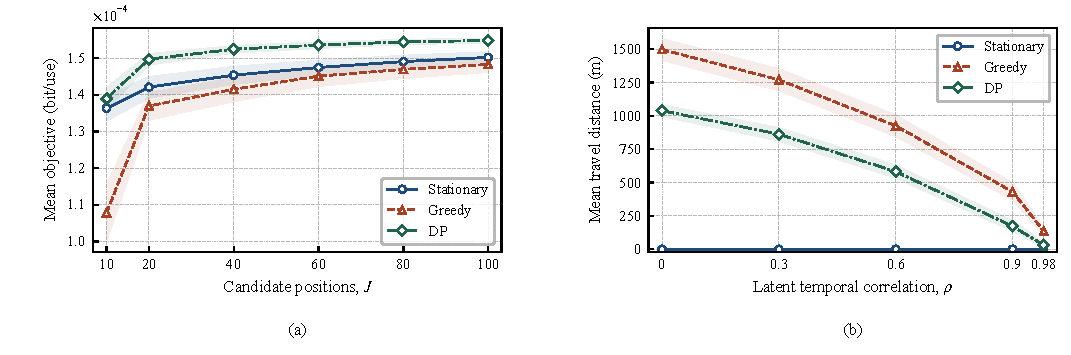
\includegraphics[width=\textwidth]{figures/fig3_parameter_sensitivity.pdf}
\caption{Sensitivity at $\lambda_{\rm ref}$: (a) mean penalized objective
versus candidate positions; (b) mean travel distance versus latent cloud
correlation. Shaded bands show pointwise 95\% intervals over 100 missions.}
\label{fig:temporal}
\label{fig:sensitivity}
\end{figure*}

Fig.~\ref{fig:sensitivity}(a) shows that increasing $J$ from 10 to 100
improves mean DP objective by 11.409\%. Nested position sets enlarge
the feasible space, so optimal P2/DP objectives cannot decrease.
The $J=10$ graph has eight connected components; the initial improvement
therefore includes connectivity as well as additional spatial choices.
As observed in Fig.~\ref{fig:sensitivity}(b), increasing $\rho$ from
0 to 0.98 reduces mean DP distance from 1038.25 to 31.84 m.
Its relative objective advantage over Stationary falls from 23.712\%
to 0.155\%. Persistent clear locations can make offline stationary
selection competitive, an interpretation limited to the evaluated model.

The representative penalty is
$\lambda_{\rm ref}=9.468026677248516\times10^{-6}$ bit/use.
Relative to zero-penalty DP, it reduces mean travel by 88.370\% while
reducing mean usable rate by 0.515\%. At the default configuration,
DP improves mean usable rate by 4.16\%/2.70\% and mean objective by
3.07\%/4.42\% over Stationary/Greedy, respectively. All locations select
$(\nu,V_A)=(0.125,8)$ at the catalog boundary; mobility gains therefore
do not isolate shaping gain or establish continuous-source optimality.

\section{Conclusions}
\label{sec:conclusion}
Finite-catalog MB optimization of 256-QAM sources was combined with
cloud-aware stationary selection, Greedy positioning, and offline DP.
The saved results show lower observed zero-rate unavailability with DP
and substantial distance savings under a mobility penalty with a small
usable-rate loss. These findings depend on synthetic clouds, finite grids,
and future information. The retained MI--Holevo measurement mismatch
precludes a validated quantum-security claim. Future work will address
measurement-consistent security analysis, cloud prediction, and physical
UAV mobility costs.

% Generated by IEEEtran.bst, version: 1.14 (2015/08/26)
\begin{thebibliography}{1}
\providecommand{\url}[1]{#1}
\csname url@samestyle\endcsname
\providecommand{\newblock}{\relax}
\providecommand{\bibinfo}[2]{#2}
\providecommand{\BIBentrySTDinterwordspacing}{\spaceskip=0pt\relax}
\providecommand{\BIBentryALTinterwordstretchfactor}{4}
\providecommand{\BIBentryALTinterwordspacing}{\spaceskip=\fontdimen2\font plus
\BIBentryALTinterwordstretchfactor\fontdimen3\font minus
  \fontdimen4\font\relax}
\providecommand{\BIBforeignlanguage}[2]{{%
\expandafter\ifx\csname l@#1\endcsname\relax
\typeout{** WARNING: IEEEtran.bst: No hyphenation pattern has been}%
\typeout{** loaded for the language `#1'. Using the pattern for}%
\typeout{** the default language instead.}%
\else
\language=\csname l@#1\endcsname
\fi
#2}}
\providecommand{\BIBdecl}{\relax}
\BIBdecl

\bibitem{usenko2012}
V.~C. Usenko, B.~Heim, C.~Peuntinger, C.~Wittmann, C.~Marquardt, G.~Leuchs, and
  R.~Filip, ``Entanglement of gaussian states and the applicability to quantum
  key distribution over fading channels,'' \emph{New Journal of Physics},
  vol.~14, p. 093048, 2012.

\bibitem{denys2021}
A.~Denys, P.~Brown, and A.~Leverrier, ``Explicit asymptotic secret key rate of
  continuous-variable quantum key distribution with an arbitrary modulation,''
  \emph{Quantum}, vol.~5, p. 540, 2021.

\bibitem{gong2020}
S.~Gong, H.~Shen, K.~Zhao, R.~Wang, X.~Zhang, T.~de~Cola, and J.~A. Fraire,
  ``Network availability maximization for free-space optical satellite
  communications,'' \emph{IEEE Wireless Communications Letters}, vol.~9, no.~3,
  pp. 411--415, 2020.

\bibitem{usenko2016}
V.~C. Usenko and R.~Filip, ``Trusted noise in continuous-variable quantum key
  distribution: A threat and a defense,'' \emph{Entropy}, vol.~18, no.~1,
  p.~20, 2016.

\end{thebibliography}

\end{document}
